\documentclass[pdf]{beamer} % Add the [handout] option to group all of the items
\usetheme{Copenhagen}

\usepackage{pgfpages}
%\setbeameroption{show notes on second screen=right}
%\setbeameroption{show only notes}
\usepackage[utf8]{inputenc}
\usepackage[spanish]{babel}
\usepackage{paralist}
\usepackage{stmaryrd}
\usepackage{graphicx,xcolor}
\usepackage{subcaption}
\usepackage{array}
\usepackage{color}




\title{Formalización del sistema de permisos de Android 10}

\author[Universidad Nacional de Rosario]{Guido De Luca}
\institute{Universidad Nacional de Rosario}
\date{\today}

\subject{Tesina}


\begin{document}

\begin{frame}[plain]
    \titlepage
\end{frame}

\begin{frame}{Motivación}
    \begin{itemize}
        \item ¿Por qué Android? \pause Por su popularidad y alcance \pause
        \item ¿Por qué un sistema de permisos? \pause Mediador entre usuarios y aplicaciones \pause
        \item ¿Por qué métodos formales? \pause
              \begin{itemize}[<+->]
                  \item Pruebas rigurosas
                  \item Aclarar comportamientos ambiguos
                  \item Construir un framework para razonar sobre el sistema
              \end{itemize}
    \end{itemize}
\end{frame}

\begin{frame}{J.P. Anderson, 1972}
    Diseño de un mecanismo de validación por referencia:
    \pause
    \begin{itemize}[<+->]
        \item Mediación completa
        \item A prueba de manipulaciones
        \item Verificable
    \end{itemize}

    \begin{block}{Definición}
        % +1 por el \pause del principio
        \only<2>{Toda acción ejecutada por el sistema debe ser supervisada por el monitor de
            referencia.}

        \only<3>{ La ejecución del MVR no debe ser modificable manual ni programáticamente. Más
            conocido en ingles como \textit{tamper-proof}.}

        \only<4>{La implementación del validador de referencia debe ser lo suficientemente pequeña
            para ser verificable y \textit{testeable} de manera exhaustiva.}
    \end{block}
\end{frame}

\begin{frame}{Un poco de contexto sobre Android}{Arquitectura de pila}
    \begin{columns}
        \begin{column}{.6\textwidth}
            \textbf{Pila de software:} \pause
            \begin{enumerate}[<+->]
                \item Aplicaciones del sistema y de terceros
                \item \textit{API} de la plataforma
                \item Entorno de \textit{runtime} y bibliotecas nativas
                \item Capa de abstracción del hardware
                \item Núcleo de Linux
            \end{enumerate}
        \end{column}

        \begin{column}{.4\textwidth}
            \begin{figure}
                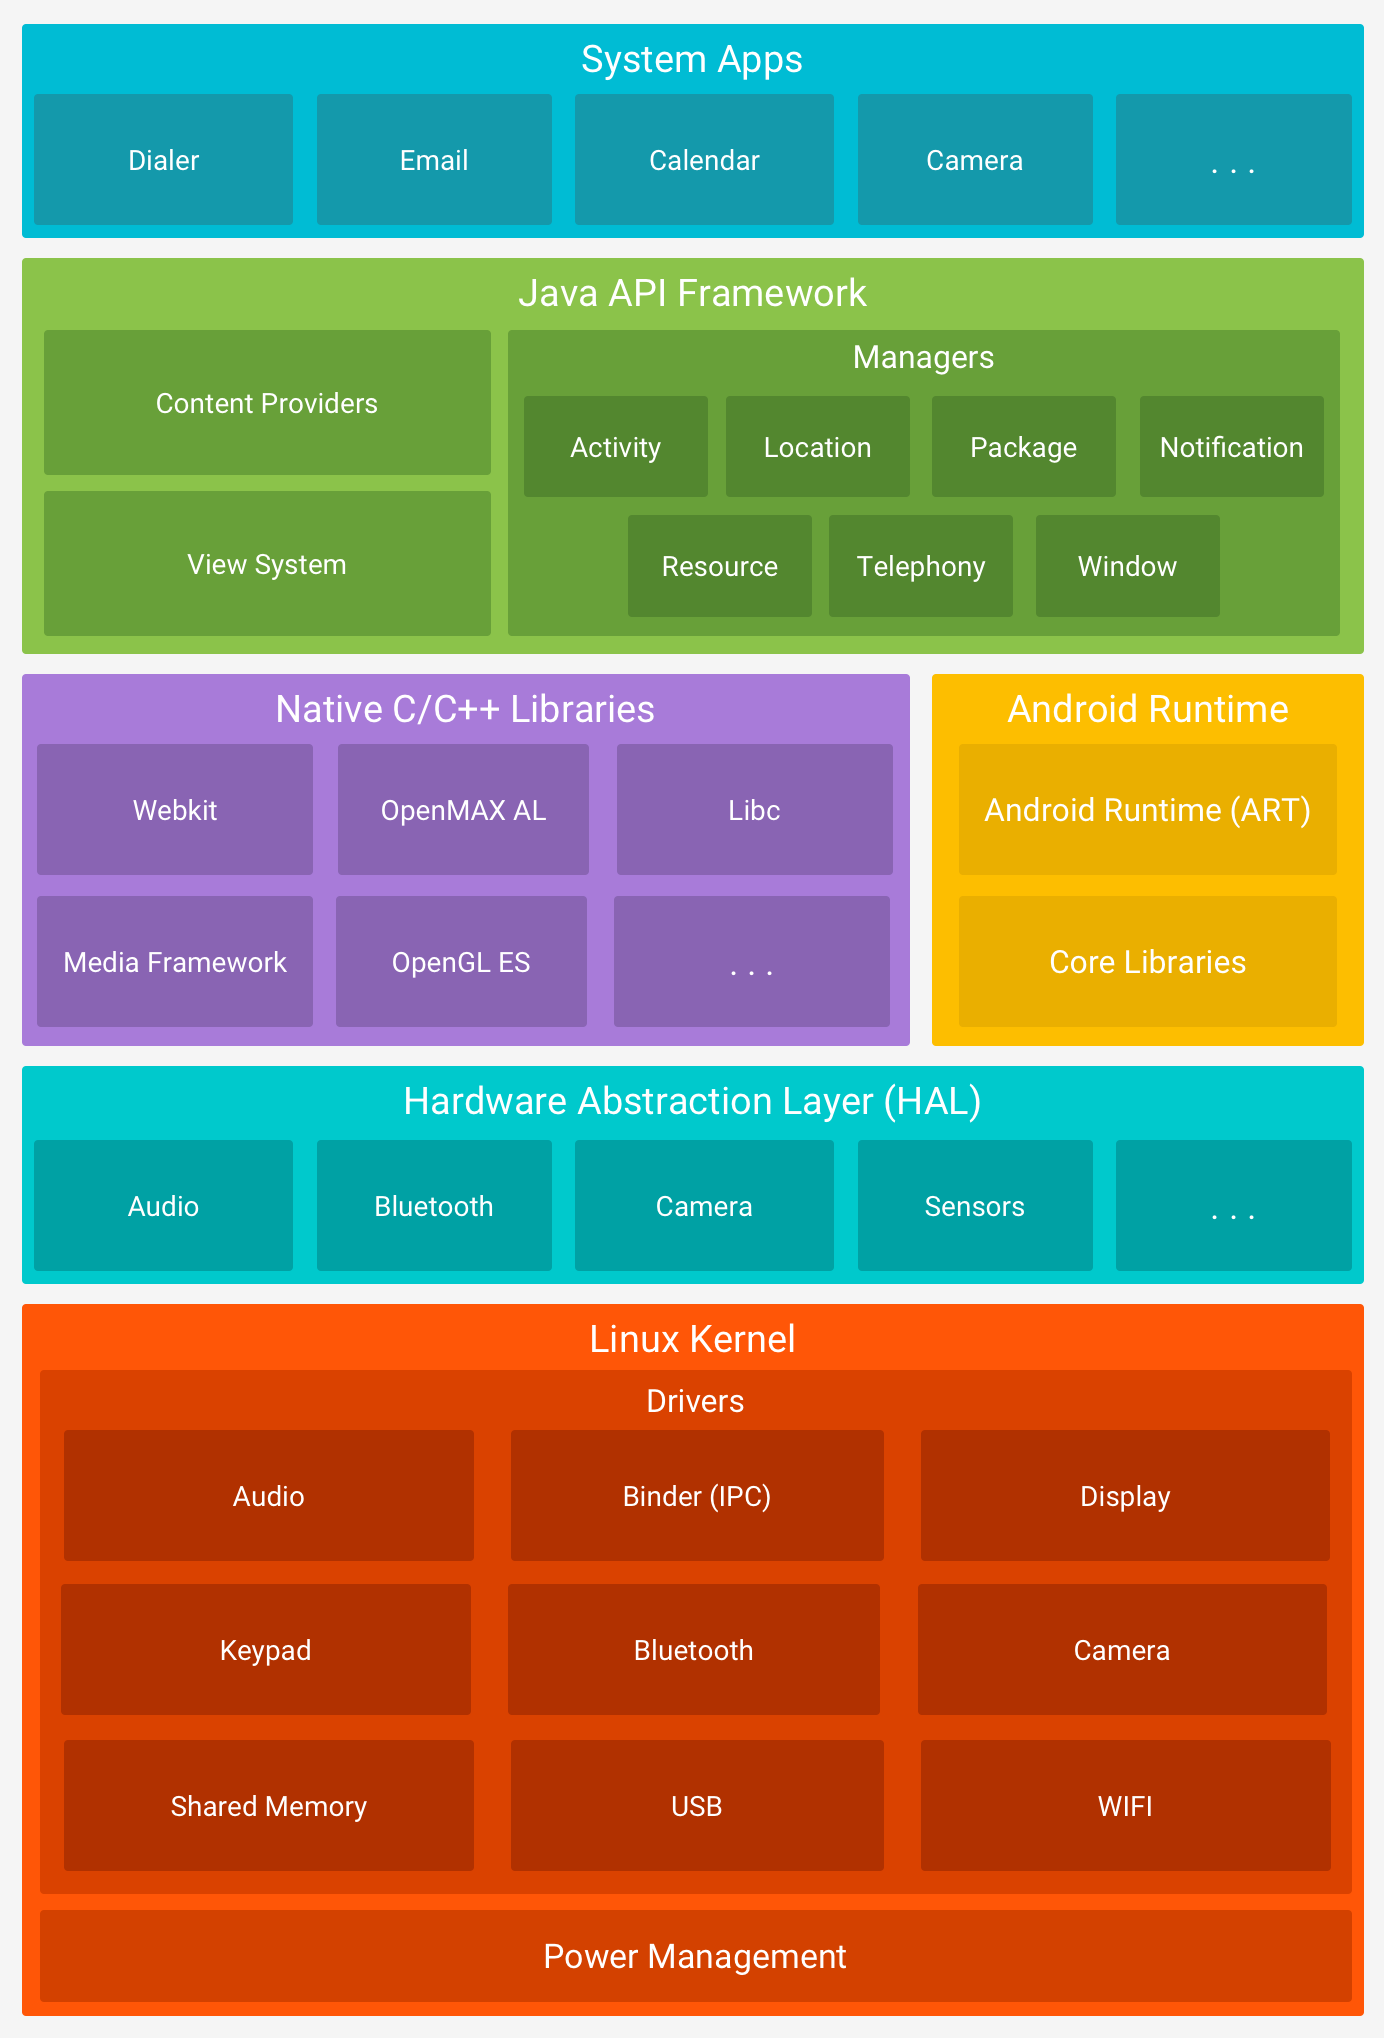
\includegraphics[scale=0.09]{../imagenes/android-stack.png}
            \end{figure}
        \end{column}
    \end{columns}
\end{frame}

\begin{frame}{Un poco de contexto sobre Android}{Componentes del sistema}
    \begin{itemize}[<+->]
        \item \textbf{Actividad}: representa una pantalla individual con interfaz de usuario
        \item \textbf{Servicio}: realiza operaciones de ejecución prolongada en segundo plano
        \item \textbf{Receptor de emisiones}: permite que el sistema u otras aplicaciones entreguen
              mensajes por fuera del flujo normal
        \item \textbf{Proveedor de contenido}: administra los datos de una aplicación para que
              puedan ser compartidos con otras
    \end{itemize}
\end{frame}

\begin{frame}{Un poco de contexto sobre Android}{Interacción entre componentes}
    \textit{Intents:} \\
    \begin{itemize}
        \item Mensajería utilizada para la comunicación entre componentes \pause
        \item Puden ser explícitos o implícitos
    \end{itemize}
    \vspace{20px} \pause
    Para recibir \textit{intents} implícitos, las aplicaciones declaran filtros de \textit{intents}.
    Este filtro se define en el \textbf{manifiesto} de la aplicación.
\end{frame}

\begin{frame}{Un poco de contexto sobre Android}{Permisos}
    Los recursos de una aplicación se protegen con distintos niveles de permisos.
    \begin{itemize}[<+->]
        \item Normal
        \item Peligrosos
        \item De misma firma
    \end{itemize}
    \vspace{20px} \pause Los permisos peligrosos se  otorgan en tiempo de ejecución. El resto, al
    instalar la aplicación.

    \vspace{20px} \pause Los permisos que pertenecen a una misma característica de una aplicación
    se agrupan en lo que definimos \textbf{grupo de permisos.}
\end{frame}

\begin{frame}{Un poco de contexto sobre Android}{Cambios de comportamiento recientes I}
    \textbf{Sistema de archivos}\\
    \vspace{10px}
    \begin{itemize}
        \item Los directorios de las aplicaciones tienen permisos restringidos
        \item Evita la fuga de metadatos
        \item Utilizar el mecanismo de \textit{intents} como la única forma segura de compartir
              archivos
    \end{itemize}
    \vspace{10px}
    \pause
    Cambio introducido en Android 7.
\end{frame}

\begin{frame}{Un poco de contexto sobre Android}{Cambios de comportamiento recientes II}
    \textbf{Cambios en permisos agrupados} \\
    \vspace{10px}
    Antes de Android 8, al otorgar un permiso peligroso, se otorgaban de manera incorrecta el resto
    de los permisos del grupo.\\
    \vspace{5px}
    A partir de esta versión de Android se corrige ese comportamiento y se define una noción de
    ``otorgamiento automático'' para permisos peligrosos.

    \vspace{10px} \pause
    \textbf{Permisos normales y peligrosos compartiendo grupo} \\
    \begin{block}{}
        ``Cualquier permiso puede pertenecer a un grupo de permisos sin importar el nivel del
        protección del mismo''
    \end{block}
    \pause
    ¿Cómo se comporta el sistema en este caso?
\end{frame}

\begin{frame}{Un poco de contexto sobre Android}{Cambios de comportamiento recientes III}
    \textbf{Chequeo de permisos en aplicaciones viejas} \\
    \vspace{10px}
    Alerta al usuario ante la ejecución de una aplicación cuyos permisos peligrosos fueron otorgados
    en tiempo de instalación.
\end{frame}

\begin{frame}{Nuestra formalización del sistema de permisos}

\end{frame}

\begin{frame}{Trabajos relacionados}
    Divididos en tres categorías:
    \pause
    \begin{itemize}[<+->]
        \item De análisis informal:
              \begin{itemize}
                  \item Características nuevas, resumen de vulnerabilidades, mitigaciones
                  \item Complemento a la documentación oficial
              \end{itemize}
        \item Herramientas de análisis estático o dinámico:
              \begin{itemize}
                  \item Sobreprivilegios, flujo indebido de la información
                  \item Estudia casos de uso específicos
              \end{itemize}
        \item De análisis formal:
              \begin{itemize}
                  \item Estudiar escenarios específicos mediante algún lenguaje formal
                  \item Especificaciones de la plataforma (en lenguajes como TLA+, Alloy, Coq)
              \end{itemize}
    \end{itemize}
\end{frame}

\begin{frame}{Conclusiones}
    \begin{itemize}[<+->]
        \item Actualizamos la formalización a una versión reciente de la plataforma
        \item Analizamos la validez de las propiedades existentes y generamos nuevas, en particular,
              relacionadas a los cambios de comportamiento de los grupos de permisos
        \item Como consecuencia de la actualización en la formalización, actualizamos la
              implementación informal  y su prueba de corrección.
    \end{itemize}
\end{frame}

\begin{frame}{Trabajo futuro}
    \begin{itemize}[<+->]
        \item Utilizar el código extraído para comparar y validar ejecuciones reales de la
              plataforma
        \item Utilizar el código extraído para generar casos de prueba
        \item Continuar actualizando la especificación con los cambios introducidos en Android 11 y
              12.
              \begin{itemize}
                  \item Reestablecimiento de permisos en aplicaciones inactivas
                  \item Permisos de un único uso
              \end{itemize}
    \end{itemize}
\end{frame}

\begin{frame}{Fin}
    \begin{center}
        \huge¡Gracias!
    \end{center}
\end{frame}

\end{document}